% !TEX root = ../apuntefinitos.tex
% !TEX encoding = UTF-8 Unicode
% !TeX spellcheck = es_ES

\part{Anexo}
\section{Solver genérico para elementos 2D (Q4)} \label{sec:q4codigo}

\begin{figure}[ht!]
	\centering
	\includegraphics[width=0.5\textwidth]{fig/q4domain.eps}
	\caption{Problema plane-stress a resolver. $F=10$kN, $t=1$cm.}
\end{figure}

\lstinputlisting[caption = {q4shapefun.m}]{code/q4shapefun.m}
\clearpage
\lstinputlisting[caption = {q4solve.m}]{code/q4solve.m}
\lstinputlisting[caption = {q4stress.m}]{code/q4stress.m}
\lstinputlisting[caption = {q4graphstress.m}]{code/q4graphstress.m}
%set(gcf,'renderer','Painters');filename='q4domain';
%print('-depsc','-tiff','-r300', '-painters',[filename,'.eps'])
\clearpage
\begin{figure}[ht!]
	\centering
	\includegraphics[width=0.5\textwidth]{code/q4domain.eps}
	\vspace{-1cm}
	\caption{Resultado de los códigos de la sección \ref{sec:q4codigo}. }
\end{figure}

\section{Cuadratura de Gauss}
\lstinputlisting[caption = {gauss.m},label={cod:gauss}]{code/gauss.m}

\section*{Apuntes Auxiliares (Luis)}
Los elementos finitos siempre me dan soluciones más rígidas que la realidad porque estoy limitando sus nodos de movimientos mediante el uso de polinomios. En la realidad persisten funciones más complejas. Esto significa que el método de elementos finitos me aproxima la realidad por el lado más rígido, esto se tiene que tomar en cuenta!

\section*{Tablas}
\begin{table}[htb!]
	\begin{tabular}{>{$n=$}l<{ \vspace{10pt}}*{13}{c}}
		0 &&&&&&&1&&&&&&\\
		1 &&&&&&$x$&&$y$&&&&&\\
		2 &&&&&$x^2$&&$xy$&&$y^2$&&&&\\
		3 &&&&$x^3$&&$x^2y$&&$xy^2$&&$y^3$&&&\\
		4 &&&$x^4$&&$x^3y$&&$x^2y^2$&&$xy^3$&&$y^4$&&\\
		5 &&$x^5$&&$x^4y$&&$x^3y^2$&&$x^2y^3$&&$xy^4$&&$y^5$&\\
		6 &$x^6$&&$x^5y$&&$x^4y^2$&&$x^3y^3$&&$x^2y^4$&&$xy^5$&&$y^6$
	\end{tabular}
	\caption{El triangulo de pascal de orden $n=6$.}
\end{table}
\begin{table}[htb!]
	\centering
	\begin{tabular}{ll}
		\hline
		\multicolumn{2}{c}{Factor Corrección para $\nu\approx0,25$}                             \\ \hline
		Perfil                                                   & $k$                             \\ \hline
		Rectangular $\frac{h}{b}\gtrsim1$                        & $\frac{5}{6}$                   \\
		Rectangular $\frac{h}{b}=0,5$                            & $0,7961$                        \\
		Rectangular $\frac{h}{b}=0,25$                           & $0,6308$                        \\
		Circular                                                 & $\frac{9}{10}$                  \\
		Tubo de paredes delgadas circular                        & $\frac{1}{2}$                   \\
		\multicolumn{1}{c}{\multirow{2}{*}{Wide Flange doble T}} & $k_y\approx \frac{A_f}{1,2 A}$ \\
		\multicolumn{1}{c}{}                                     & $k_z\approx \frac{A_w}{ A}$  \\ \hline 
	\end{tabular}
	\caption{$A_w$ es el área del alma y $A_f$ es el área del ala.}
	\label{tab:kcorrectionfactor}
\end{table}

\section*{Expresiones útiles}
Operador derivada
\begin{itemize}
	\item Barra: $\partial x$
	\item Viga: $\dpartial{v}{x}$
	\item 2D: $\begin{bmatrix}
	\partial/\partial x & 0\\
	0 & \partial/\partial y \\
	\partial/\partial y & \partial/\partial x
	\end{bmatrix}$
	
\end{itemize}

\begin{align}
\sigma_{v}&=\sqrt{\sigma_{x}^2+\sigma_{y}^2+\sigma_{z}^2 - \sigma_x \sigma_y-\sigma_x\sigma_z -\sigma_y \sigma_z +3(\sigma_{xy}^2+\sigma_{xz}^2 +\sigma_{yz}^2)} \\
\sigma_{v}&=\sqrt{\tfrac{1}{2}\left[  (\sigma_{11}-\sigma_{22})^2+(\sigma_{11}-\sigma_{33})^2+(\sigma_{22}-\sigma_{33})^2\right] +3(\sigma_{12}^2+\sigma_{13}^2 +\sigma_{23}^2)}
\end{align}

\begin{equation}
\lambda = \frac{E \nu}{(1+\nu)(1-2\nu)} \qquad\quad \mu=G=\frac{E}{2(1+\nu)}
\end{equation}

\begin{equation}
\begin{bmatrix}
\sigma_{xx} \\
\sigma_{yy} \\
\sigma_{xy}
\end{bmatrix}
={\frac{E}{1-\nu^2}} 
\begin{bmatrix}
1 & \nu & 0 \\
\nu & 1 &0 \\
0 & 0 & \frac{1-\nu}{2}
\end{bmatrix}
\cdot
\begin{bmatrix}
\varepsilon_{xx} \\
\varepsilon_{yy} \\
2\varepsilon_{xy}
\end{bmatrix}
\end{equation}

\begin{equation}
\begin{bmatrix}
\sigma_{11} \\
\sigma_{22} \\
\sigma_{12}
\end{bmatrix}
={\frac{E}{(1+\nu)(1-2\nu)}} 
\begin{bmatrix}
1-\nu & \nu &0 \\
\nu &1-\nu& 0 \\
0 & 0 & \frac{1-2\nu}{2}
\end{bmatrix}
\cdot
\begin{bmatrix}
\varepsilon_{11} \\
\varepsilon_{22} \\
2\varepsilon_{12}
\end{bmatrix}
\end{equation}

\begin{equation}
\sigma_{n}=\frac{\sigma_{xx}+\sigma_{yy}}{2}+\left(\frac{\sigma_{xx}-\sigma_{yy}}{2}\right)\cos 2\theta +\tau_{xy}\sin 2\theta 
\end{equation}

\begin{equation}
\tau_{n}=-\left(\frac{\sigma_{xx}-\sigma_{yy}}{2}\right)\sin 2\theta +\tau_{xy}\cos 2\theta 
\end{equation}

\begin{equation}
I=\int^1_{-1} \phi(\xi) \di \xi \approx \phi(\xi_1) W_1+\phi(\xi_2) W_2 \ldots \phi(\xi_n) W_n
\end{equation}
\begin{equation}
I=\int^1_{-1} \int^1_{-1}\phi(\xi,\eta) \di \xi \di \eta\approx \sum_i \sum_j W_i W_j\phi(\xi,\eta) 
\end{equation}

Se suele requerir que $\eta\leq 0,05$


Formulación de elemento rígido RBE2:

\begin{align*}
g_u = u_{s}-u_{m}+L_{e}\versor{v}_{y}\,\left(\frac{\theta_{m}\,\sin\left(\sqrt{\squareangles}\right)}{\sqrt{\squareangles}}+\frac{\varphi_{m}\,\psi_{m}\,\left(\cos\left(\sqrt{\squareangles}\right)-1\right)}{\squareangles}\right)-&L_{e}\versor{v}_{z}\,\left(\frac{\psi_{m}\,\sin\left(\sqrt{\squareangles}\right)}{\sqrt{\squareangles}}-\frac{\varphi_{m}\,\theta_{m}\,\left(\cos\left(\sqrt{\squareangles}\right)-1\right)}{\squareangles}\right)\\
- \frac{L_{e}\versor{v}_{x}\,\left({\psi_{m}}^2+{\theta_{m}}^2\right)\,\left(\cos\left(\sqrt{\squareangles}\right)-1\right)}{\squareangles}
\end{align*}

\begin{align*}
g_v = v_{s}-v_{m}-L_{e}\versor{v}_{x}\,\left(\frac{\theta_{m}\,\sin\left(\sqrt{\squareangles}\right)}{\sqrt{\squareangles}}-\frac{\varphi_{m}\,\psi_{m}\,\left(\cos\left(\sqrt{\squareangles}\right)-1\right)}{\squareangles}\right)+&L_{e}\versor{v}_{z}\,\left(\frac{\varphi_{m}\,\sin\left(\sqrt{\squareangles}\right)}{\sqrt{\squareangles}}+\frac{\psi_{m}\,\theta_{m}\,\left(\cos\left(\sqrt{\squareangles}\right)-1\right)}{\squareangles}\right)\\ -\frac{L_{e}\versor{v}_{y}\,\left({\varphi_{m}}^2+{\theta_{m}}^2\right)\,\left(\cos\left(\sqrt{\squareangles}\right)-1\right)}{\squareangles}
\end{align*}

\begin{align*}
g_w = w_{s}-w_{m}+L_{e}\versor{v}_{x}\,\left(\frac{\psi_{m}\,\sin\left(\sqrt{\squareangles}\right)}{\sqrt{\squareangles}}+\frac{\varphi_{m}\,\theta_{m}\,\left(\cos\left(\sqrt{\squareangles}\right)-1\right)}{\squareangles}\right)-&L_{e}\versor{v}_{y}\,\left(\frac{\varphi_{m}\,\sin\left(\sqrt{\squareangles}\right)}{\sqrt{\squareangles}}-\frac{\psi_{m}\,\theta_{m}\,\left(\cos\left(\sqrt{\squareangles}\right)-1\right)}{\squareangles}\right) \\  - \frac{L_{e}\versor{v}_{z}\,\left(\cos\left(\sqrt{\squareangles}\right)-1\right)\,\left({\varphi_{m}}^2+{\psi_{m}}^2\right)}{\squareangles}
\end{align*}

donde \(\vartheta = \varphi_m^2 + \psi_m^2 + \theta_m^2\)


\begin{equation*}
g_\varphi = \varphi_s - \varphi_m\, , \qquad g_\psi = \psi_s - \psi_m\, , \qquad g_\theta = \theta_s - \theta_m
\end{equation*}


En 2D


\clearpage
\section*{Figuras}
\begin{figure}[htb!]
	\centering
	\includegraphics[width=0.5\textwidth]{fig/pascalsTetra.eps}
	\caption{El tetraedro de Pascal. Los términos de los elementos \textit{serendipidad} están encuadrados.}
	\label{fig:PascalsTetrahedron}
\end{figure}

\begin{figure}[htb!]
	\centering
	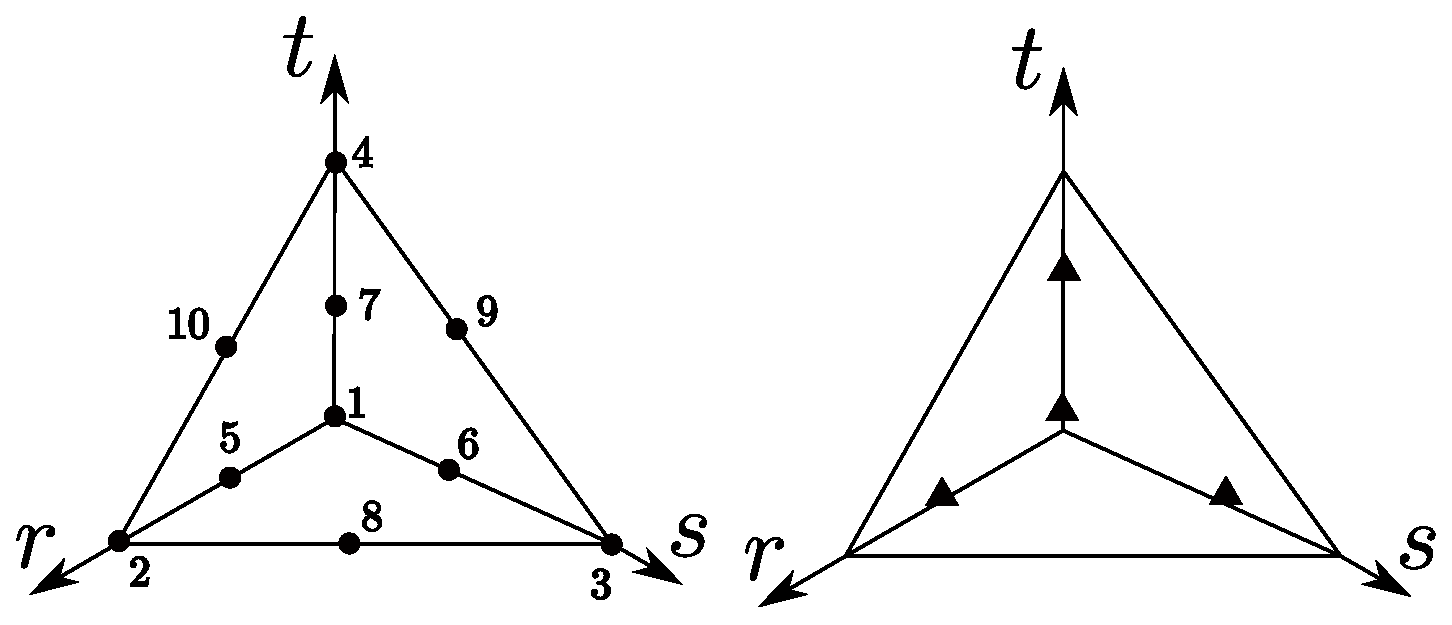
\includegraphics[width=0.8\textwidth]{fig/T10numbering.eps}
	\caption{Numeración de un tetraedro de diez nodos y la ubicación de los puntos Gauss para un grado de precisión 2.}
	\label{fig:T10numbering}
\end{figure}



% \begin{comment}
%     \section{Dudas}
%     \begin{enumerate}
%         \item Pg. 223 Cook: $\Mk$ de un solido 8 nodos se integra con $n=2$, pero $\MB$ se integra con $n=3$. Pero se necesita $\MB$ para obtener $\Mk$.
%         \item Si quiero verificar calidad de un elemento, me basta con pararme arriba cada punto Gauss y verificar que $\Djac$ no sea igual a cero y que no cambie de signo?
%         \item Tengo un problema plain strain pero tengo $q(x)$ en [N/m]. No lo integro con $t$! No? Inversamente, para el mismo problema, si tengo solo presiones o fzas volumetricas puedo olvidarme que existe $t$ y no usarla para el calculo de la matriz rigidez (y presiones/fzas vol). Se le dice singularidad a un punto donde $\Djac$ es cero
%         \item Si quiero tensiones en puntos Gauss, cambia la dimension de $\MB$ cuando itero sobre los puntos? Cook dice que $\MB$ is calculated from (lower order) displacement field. wtf?
%         \item \textbf{Follow-up} Cuando itero sobre los mismos Puntos de Gauss para obtener tensiones, cambian mis $\MN$? Sé que puedo usar los puntos de Gauss para extrapolar tensiones en los nodos, pero hablo antes de eso
%         \item Para un elemento me conviene siempre ser perfectamente simétrico en la elección del orden del polinomio? Hay alguna vez que voy a tomar $[1\ms x\ms y\ms xy\ms x^2]$ antes de tomar algo por el estilo de  $[1\ms x\ms y\ms y^2\ms x^2]$
%     \end{enumerate}
%     \end{comment}

